\chapter{A Closer Look at Scoring}
\label{ch:scoring}
% ##################################################################################################################

\hfill \textbf{Author:} Andreas Horni, Kai Nagel

\begin{center} 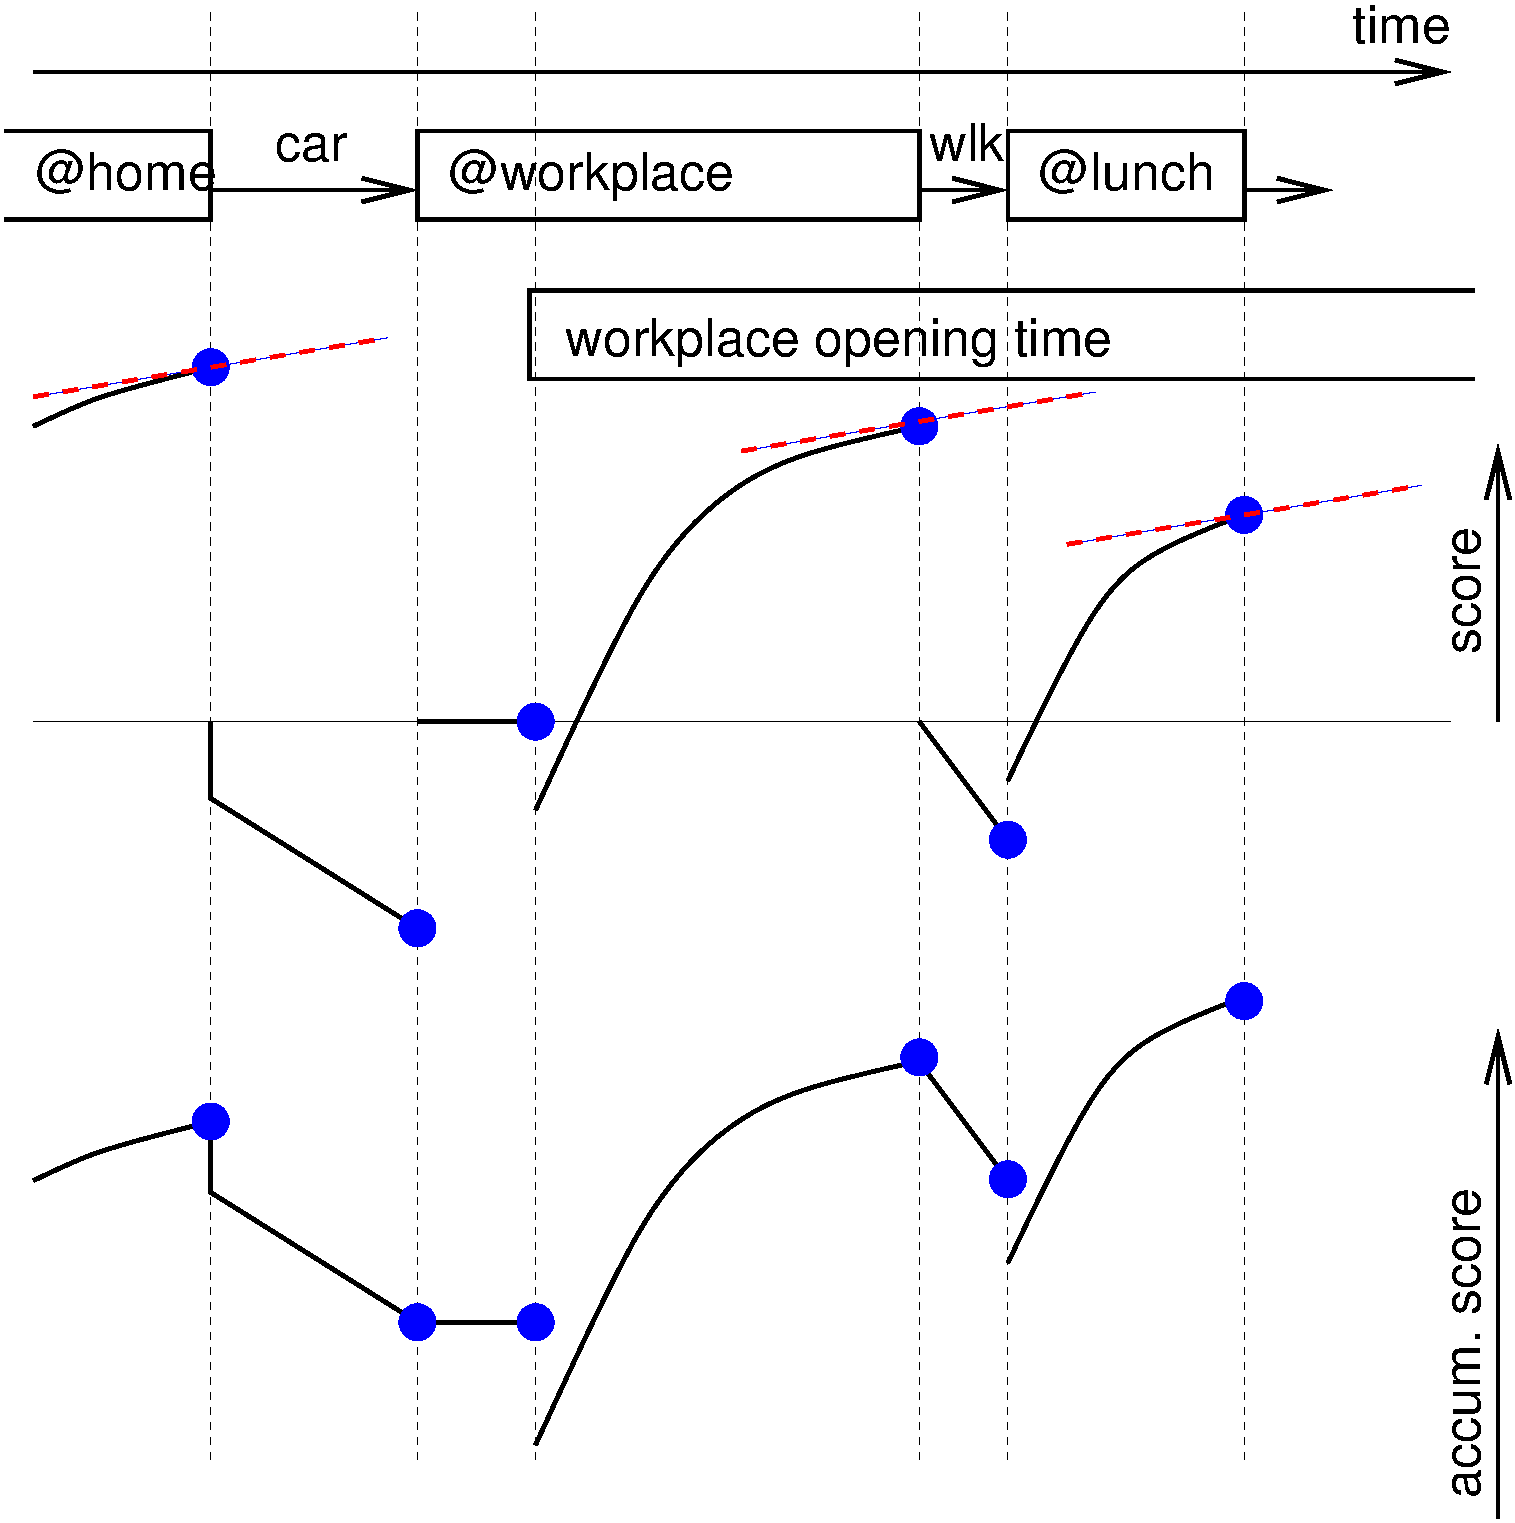
\includegraphics[width=0.3\textwidth, angle=0]{using/figures/scoring-example} \end{center}

% ##################################################################################################################

\section{Good Plans and Bad Plans, Score and Utility}

\kai{im folgenden habe ich noch ein paar Absätze neu geschrieben, muss daher doppelt gründlich durchgeschaut werden}

As outlined in Section~\ref{sec:co-ev} and by Figures~\ref{fig:matsimcycle} and~\ref{fig-ea}, \gls{matsim} is based on a co-evolutionary algorithm where each individual agent learns by maintaining multiple plans which are scored by executing them in the mobsim, selected according to the score, and sometimes modified.  Somewhat more detailed, the iterative process contains the following elements:
%
\begin{description}
\item[mobsim] The mobility simulation takes one ``selected'' plan per agent and executes it in a synthetic reality.  This may also be called network loading.

\item [scoring] The actual performance of the plan in the synthetic reality is taken to compute the each executed plan's score.

\item [replanning] consists of several steps:
  \begin{enumerate}

  \item If an agent has more plans than the maximum number of plans (a configuration parameter), then plans are removed according to a (configurable) plan selector (choice set reduction/plans removal).

    \item For some agents, a plan copied, modified, and then selected for the next iteration (choice set extension/innovation).

  \item All other agents select between their plans (choice).
  \end{enumerate}
\end{description}

The plans of an agent in a given iteration may be considered the agent's \imp{choice set} in that iteration.  In consequence, steps~1 and~2 of replanning are modifying the choice set, while step~3 implements the actual \imp{choice} between options.
%
Choice is typically based on the score, with plans with a higher score having a higher probability of being selected.  
%
This is dicussed in more detail in Chapter~\ref{ch:abta}.  For the time being, note that the three steps of replanning need to cooperate for the approach to work: The plans removal step should remove ``bad'' plans, and the innovation step should generate ``good'' plans, where in both cases ``good'' means ``being able to obtain a high score in the mobsim/scoring''.  Fortunately, the approach, due to its evolutionary concept, is fairly robust: The innovation step does not always have to generate good solutions; it is sufficient if \emph{some} of the solutions are good ones that lead to a high score.

However, from the above it should become clear that scoring is a central element of \gls{matsim}.  Only solutions that obtain a high score will be selected by the agent, and will survive the plans removal step.  In consequence, the scoring function needs to be ``correct'' for a given scenario, which roughly means that plans ``perform well'' obtain a higher score than plans that do ``not perform well''.  And if a performance is good or not is in the end decided by the persons living in a region -- some persons may prefer a congested car trip to a destination, some others may prefer a crowded but affordable trip by public transit, while even others may prefer using the bicycle even in bad weather.

The typical way to bridge this gap is to use econometric \imp{\gls{utility}} functions, for example from random utility models \citep[e.g.][]{BenAkivaLerman_1985,Train_2003} for the score.  However, in \gls{ai} utility may also be used in a more general way, as the \gls{score} that either each individual agent or the system as a whole wants to or should optimize \citep{RusselNorvig2010ArtificialIntelligence}.  \kai{Etwas davon sollte wohl auch ins Glossar.} For those reasons, the terms ``\gls{score}'' and ``\gls{utility}'' are mostly interchangeable in the \gls{matsim} context.  Since at some places we will need the concept of a marginal utility, this chapter will mostly speak of utility since it feels a bit unusual to speak of marginal score.

The user has the possibility to configure numerous parameters to calibrate the
%choice behavior.
scoring function.
%scoring function und choice behavior sind nicht identisch: zu letzterem gehört auch das Austauschen von ExpSelectBeta gegen SelectBest oder so.
When users are ready to extend \gls{matsim} in the next book part, they will also learn how to plug in their own customized scoring function.

%% \gls{matsim} is based on \gls{utility}-maximization. Thus, estimated discrete choice models can be applied in \gls{matsim}. However, because of \gls{matsim}'s iterative 
%% structure, and
However, because \gls{matsim} it is based on complete day plans, the application of choice models for parts of day plans only (for example mode choice) is not straight forward, as detailed in Section~\ref{sec:estimation}.
%
% "due to" vs "because of" see http://web.ku.edu/~edit/because.html
%
Because of the absence of complete-day-utility functions in the literature, \gls{matsim} has
%been
started with the so-called Charypar-Nagel scoring or \gls{utility} function (Section~\ref{sec:charyparnagel}).  Sometimes, this scoring function was modified, extended, or replaced for specific investigations (Section~\ref{sec:appsExtensions}). Readily applicable estimates for a full-day utility function are not yet available as discussed in Section~\ref{sec:estimation}.

% ##################################################################################################################
\section{The Current Charypar-Nagel Utility Function}
\label{sec:charyparnagel}
% ============================================================================================
\subsection{Mathematical Form}
\label{sec:mathematical-form}

The first and still basic \gls{matsim} scoring function was formulated by \citet[][]{CharyparNagel2005ga4acts} loosely based on the \emph{Vickrey} model for road congestion as described in \citet[][]{Vickrey_TAER_1969} and \citet[][]{ArnottEtAl_TAER_1993}. Originally, this formulation was established for departure time choice. However, all studies performed so far indicate that the \gls{matsim} function is also appropriate for modeling 
%the
further choice dimensions.
%
It is, however, almost certainly not appropriate for activity dropping and activity addition (see Section~\ref{sec:scoring-current}).

%% As in the discrete choice modeling framework (see Chapter~\ref{ch:discretechoice}), the utility $S_{}$ is composed of a deterministic part $V$ and a random error term $\varepsilon$, i.e., $S_{} = V_{} + \varepsilon$. Except for destination choice the error term is not explicitly generated but stems from the random noise produced by the co-evolutionary process.  \kai{(*)}  Randomness is added in various ways in the process, an example is the order in which agents undergo the replanning (e.g., in which iteration choices are modified). \ah{Hier Diskussion Section~\ref{sec:discussion_scoring} noch weiter vertiefen}.

%% \kai{Andreas, die Aussage (*) stimmt so leider nicht.  Zum einen \emph{erzeugt} die Simulation Noise (wie Du schreibst), zum anderen \emph{parametrisiert} das Logit-Modell (wenn eingestellt) weiteren Noise.  Dies vor allem bei VSP; ihr seid ja weitgehend bei SelectBest geblieben, was sich hier als die theoretisch bessere Lösung herausstellt.}

%% \kai{Noch besser wäre es vermutlich, Deinen Ansatz mit den ``frozen epsilons'' breiter anzuwenden.}

% -------------------------------------------------------------------------------------
\paragraph{Basic Function}

For the basic function, the utility of a plan $S_{plan}$ is computed as the sum of all activity utilities $S_{act,q}$ plus the sum of all travel (dis)utilities $S_{trav,mode(q)}$:
%
\begin{equation}
\label{eq:matsimUTF}
S_{plan}=\sum^{N-1}_{q=0} S_{act,q} + \sum^{N-1}_{q=0} S_{trav, mode(q)}
\end{equation}
with $N$ as the number of activities. Trip $q$ is the trip that follows activity $q$. The last activity is for scoring merged with the first activity, thus there is an equal number of trips and activities.
%does not have an associated trip, thus the sum goes only up to $N-1$.  
%\kai{Andreas, Macht Ihr das so?  Die Standard-Variante, die auch am VSP verwendet wird, "näht" die erste und die letzte Aktivität zusammen.  Damit haben wir genauso viele Aktivitäten wie Trips.}
%\ah{dann lag ich hier wohl falsch. korrigiert.}

% -------------------------------------------------------------------------------------
\paragraph{Activities}

\kai{Andreas, there are no separate beta parameters per activity type.  maybe it would make sense to have them in some cases, but this would be a somewhat larger software change since at this point we cannot attach them to the activity types.}

The utility of an activity $q$ is defined as follows \citep[see also][p.377ff]{CharyparNagel2005ga4acts}:
\begin{equation}
S_{act,q} = S_{dur,q} + S_{wait,q} + S_{late.ar,q} + S_{early.dp, q} + S_{short.dur, q},
\label{eq:matsimUTFact}
\end{equation}
where:
\begin{itemize}
\item $S_{dur,q}= \beta_{dur} \cdot t_{typ,q} \cdot \ln(t_{dur,q}/t_{0,q})$ 
%
is the utility of performing activity $q$, where opening times of activity locations are taken into account. $t_{dur,q}$ is performed activity duration, $\beta_{dur}$ is the marginal utility of activity duration (or marginal utility of time as a resource---the same for all activities),
% for its typical duration $t_{typ,q}$, 
and $t_{0,q}$ is minimal duration, or in other words, the duration for which utility starts to be positive. 
%
%\kai{Andreas, betaPerf gibt es (absichtlich) nur einmal, und nicht pro Aktivitätentyp.  Unterschiedlicher Zeitdruck kann sich immer noch ergeben, weil EQ~(\ref{eq:mUTTSfull}) für Akvitiäten innerhalb eines bestimmten Zeitfensters höher sein kann (weil dann für diese Aktivitäten $t_{dur,q}$, wg.\ Zeitknappheit, relative gesehen kürzer ist).}  
%%
%\ah{got it}
%
\item $ S_{wait,q} = \beta_{wait} \cdot t_{wait,q}$ 
%
denotes the waiting time spent for example in front of a yet closed store; $\beta_{wait}$ is the \emph{direct} marginal utility of time spent waiting which should \emph{not} contain the marginal utility of time as a resource $\beta_{dur}$ from above; and $t_{wait,q}$ is the waiting time.
%
It is recommended to leave $\beta_{wait}$ at zero; also see Section~\ref{sec:schedule-delay-costs}.

\item $S_{late.ar,q}= \left\{
  \begin{array}{l l}
    \beta_{late.ar} \cdot (t_{start,q} - t_{latest.ar,q}) & \quad \text{if $t_{start,q} > t_{latest.ar,q}$}\\
    0 & \quad \text{else}
  \end{array} \right.$
%  
  specifies the late arrival penalty, where $t_{start,q}$ is the starting time of activity $q$ and $t_{latest.ar}$ is the latest possible starting time of that activity for example given by opening times.
%
\item $S_{early.dp} = \left\{
  \begin{array}{l l}
    \beta_{early.dp} \cdot (t_{earliest.dp, q} - t_{end,q}) & \quad \text{if $t_{end,q} > t_{earliest.dp,q}$}\\
    0 & \quad \text{else}
  \end{array} \right.$
%
defines the penalty for staying not long enough, where $t_{end,q}$ is the ending time of the activity and $t_{earliest.dp,q}$ is the earliest possible end time for activity $q$.
%
\item $ S_{short.dur, q} = \left\{
  \begin{array}{l l}
    \beta_{short.dur} \cdot (t_{short.dur, q} - t_{dur,q}) & \quad \text{if $t_{dur,q} < t_{short.dur,q}$}\\
    0 & \quad \text{else}
  \end{array} \right.$
%  
  is the penalty for a too short activity, where $t_{short.dur}$ is the shortest possible duration for the activity.
\end{itemize}

\paragraph{Travel} 

\kai{Andreas, the mode-dependent beta can only be specified by mode, but not by the number of the trip or leg, \ie not by q.  I changed all ``q'' to $mode(q)$.}

Travel disutility for a leg $q$ is given as 
\begin{equation}
\label{eq:tdisutility}
\begin{matrix}
S_{trav, q} & = & C_{mode(q)} + \beta_{trav, mode(q)} \cdot t_{trav, q} + \beta_{m} \cdot \Delta m_q \\
& & + (\beta_{d, mode(q)} + \beta_{m} \cdot \gamma_{d, mode(q)}) \cdot d_{trav,q} 
%
+ \beta_{transfer} \cdot x_{transfer,q} \, \\
\end{matrix}
\end{equation} 
where:
%
\begin{compactitem} 
\item $C_{mode(q)}$ is a mode-specific constant,
\item $\beta_{trav, mode(q)}$ is the \emph{direct} marginal utility of time spent traveling by mode (normally negative or zero); it should \emph{not} contain the marginal utility of time as a resource $\beta_{dur}$ from above,
\item $t_{trav, q}$ is the travel time between location of activity $q$ and $q+1$,
\item $\beta_{m}$ is the marginal utility of money (normally positive),
\item $\Delta m_q$ is the change in the monetary budget invoked by fares or tolls for the complete leg (normally negative or zero),
\item $\beta_{d, mode(q)}$ is the  marginal utility of distance (normally negative or zero),
\item $\gamma_{d, mode(q)}$ is the mode-specific monetary distance rate (normally negative or zero),
\item $d_{trav, q}$ is the distance traveled between location of activity $q$ and $q+1$, 
\item $\beta_{transfer}$ are transfer penalties in public transport (normally negative),
%\kai{is this mode-specific?}\kai{no it is not}, 
and
\item $x_{transfer,q}$ is a 0/1 variable denoting if a transfer has happened between the previous and the current leg.
\end{compactitem}
%
\benjamin{Irgendwo müsste dann definiert werden, was ``direct'' vs ``indirect'' ist; M.E. einfach ``without'' vs ``with'' (time) costraints.}
%
This is the direct utility contribution of travel; see Section~\ref{sec:opport-cost-of-time} for the the full indirect utility as well as the relation to the \gls{vtts}, and Section~\ref{ch:economicEval} for a more general discussion.

Note that the distance contributes to disutility in two ways. First, it is included in a direct manner via $\beta_{d, mode(q)}$, which is natural for modes with physical efforts such as walking or cycling. Second, distance is also included monetarily via $\beta_m \cdot \gamma_{d, mode(q)}$ which is natural for mode car or pt, where monetary costs increase dependent on distance. \benjamin{Maybe add: `The current specification makes it possible to use either of those approaches for each transport mode'}.

%% \kai{distance both via distance cost rate and via direct marginal utl.  ok with me, BK will (probably) be less happy. If it stays this way, config needs to be made consistent with text above.}

%% \ah{Hatte, glaube ich, aus dem User Guide abgeguckt.}

%Ist jetzt im code nicht mehr deprecated. kai, dec'14

% ------------
\createfigure[!h!]%
{Illustration of the scoring function.}%
{Illustration of the scoring function. TOP: Individual contributions of the activities and legs.  BOTTOM: Score accumulation over the day \ah{act starts negative, thus, acc score should start with a negative offset, right? thx Marcel!}}%
{\label{fig:scoring-function}}%
{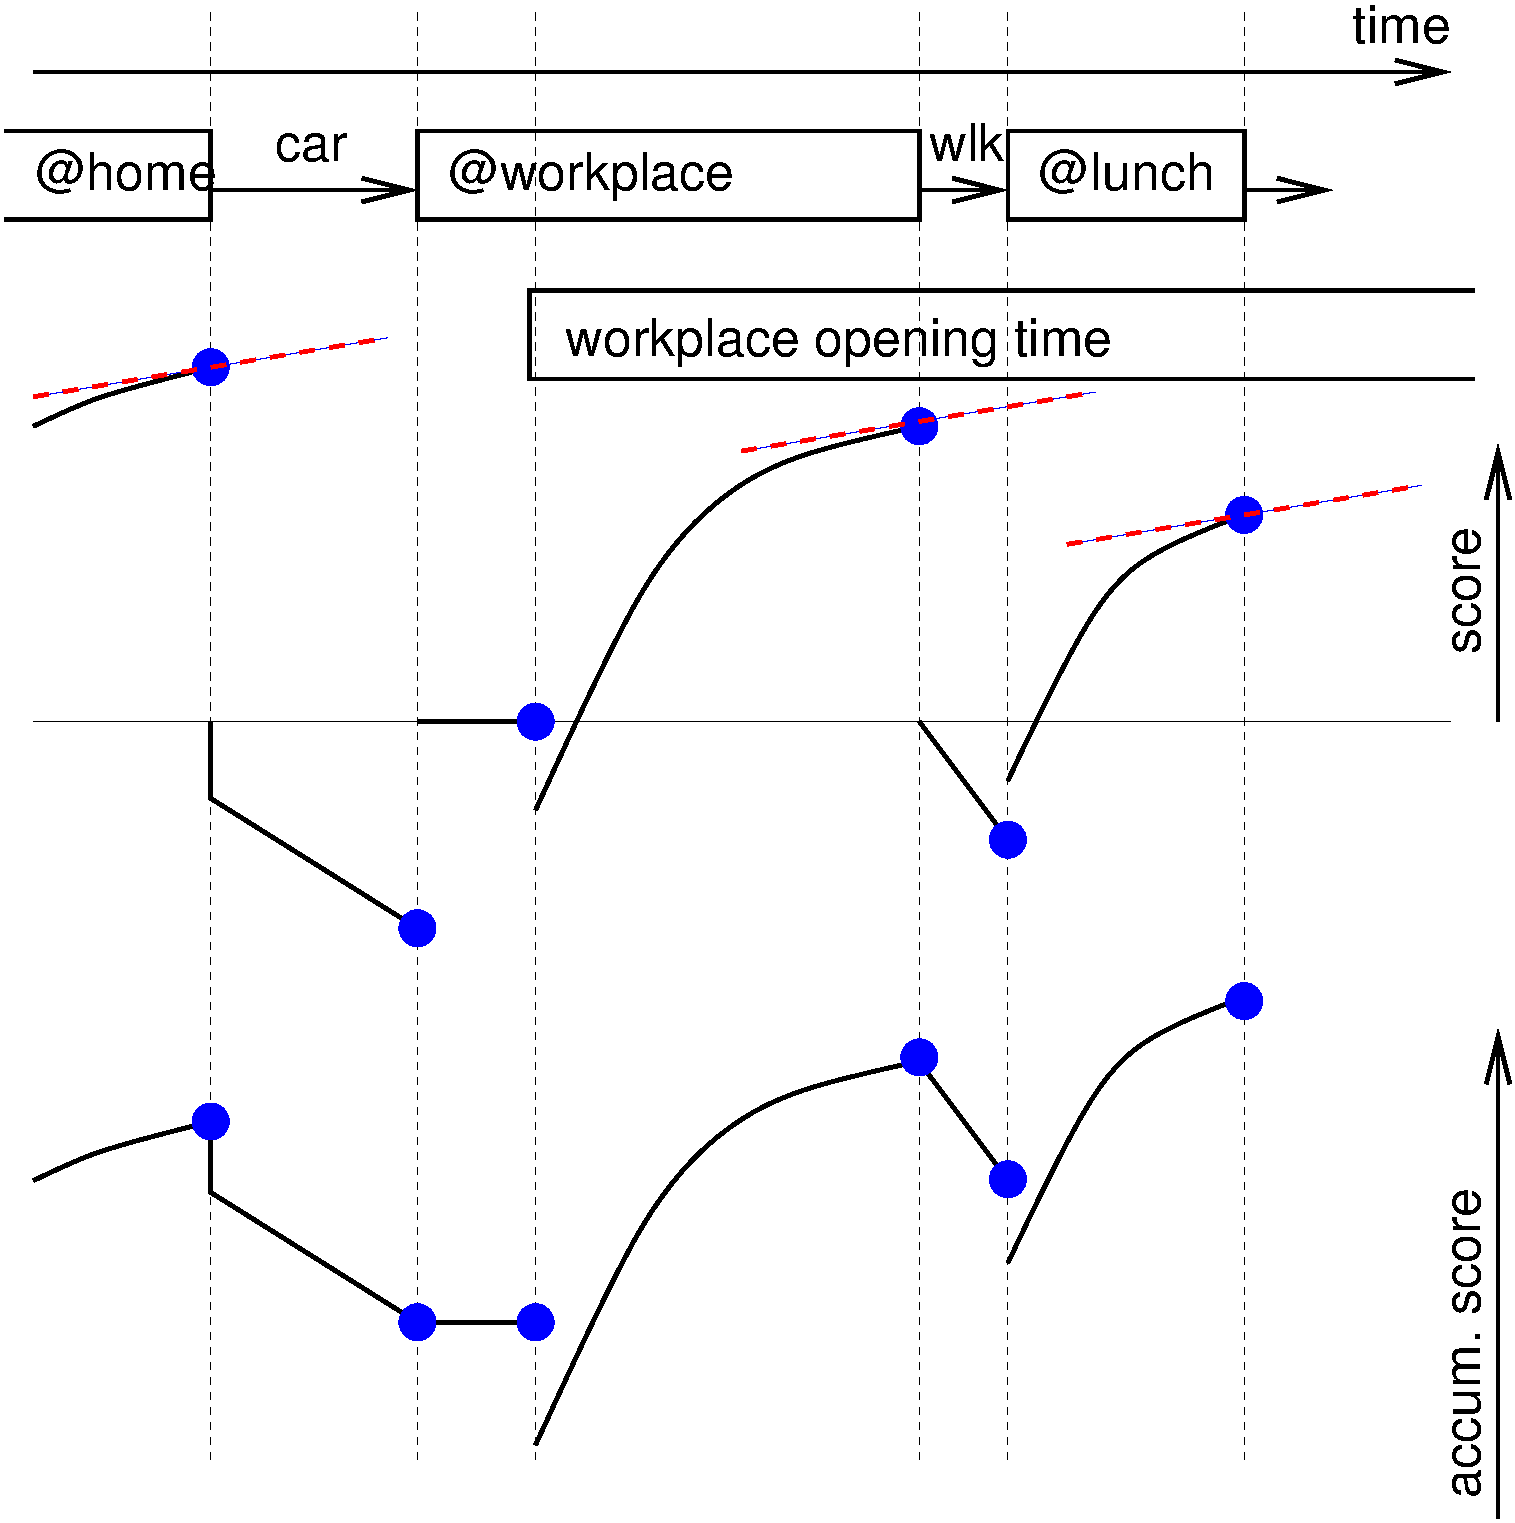
\includegraphics[width=0.8\hsize,trim=0 0 0 0,clip]{using/figures/scoring-example}}%
{}
% ------------

% ====================================================================================
\subsection{Illustration}
\label{sec:utl-fct-illustration}
Figure~\ref{fig:scoring-function} illustrates the scoring function.  Time runs from left to right.  The example shows part of an executed schedule, with a home, a work, and a lunch activity, connected by a car and a walk leg.

Activities are scored with concave functions, modeling decreasing returns to spending more time at the same activity.  Travel, in contrast, is modeled with downward sloping straight lines, where the slope may be different for different modes of transport, and there may be an initial offset (alternative-specific constant).  Note the delay between the arrival at the workplace and the workplace opening time, which is reflected in no score accumulation during that period.  Agents accumulate those scores over the day, reflected in the bottom graph.

When one assumes that all other things (in particular travel times) are equal, then agents maximize their score when the activity durations are such that all activities have the same slope ($=$ the same marginal utility; red lines).  This follows from basic economic theory (\cf Section~\ref{ch:economicEval:valuingBehavior}), but can also be seen intuitively: If the red lines did not have the same slope, the agent could gain by extending those activities with steeper slope at the expense of the others.  Clearly, this holds only when all other things remain constant, in particular the travel times.

% ====================================================================================
\subsection{The ``Wrapping Around'' of the Utility Function}
\label{sec:wrap-around}
The \gls{matsim} \gls{mobsim} typically starts at midnight, and runs until all plans have reached their final activity.  That is, the \gls{mobsim} by itself is not limited to a day.  However, as already stated in Section~\ref{sec:mathematical-form}, the standard scoring function assumes that plans ``wrap around'' to 24-hour days.  In consequence, the last activity is merged with the first activity into one activity. For example, if the first activity ends at 7\,am and the last activity starts at 11\,pm, then it is assumed that this is the \emph{same} activity, with a duration of 8~hours.

Note that scoring the two activities separately would lead to a different result, because of the nonlinear (logarithmic) form of the utility of performing. For example, $\ln(1) + \ln(7) = \ln(7) \ne \ln(1 + 7) = \ln(8)$.

% ====================================================================================
\subsection{MATSim Scoring, Opportunity Cost of Time, and the VTTS}
\label{sec:opport-cost-of-time}
As a result of the wrap-around concept, travel receives, beyond the typically negative direct marginal utility $\beta_{trav, mode}$, an additional implicit penalty from the marginal opportunity cost of time: \benjamin{potentially rephrase: ``marginal utility of time as a resource''? This is more in line with the literature as we know from Section~\ref{ch:economicEval:valuingBehavior}} If a travel time could be reduced by $\Delta t_{trav}$, the person would not only gain from avoiding $\beta_{trav}~\cdot~\Delta t_{trav}$, but also from making activities longer (effect of the so-called opportunity cost of time). The \textbf{marginal \emph{utility} of travel time savings} is thus:
%
\[
mUTTS = - \frac{\partial}{\partial t_{trav}} S_{trav} + \frac{\partial}{\partial t_{dur}}S_{dur} \ .
\]
which is
\begin{equation}
mUTTS = - \beta_{trav}
%\frac{\partial}{\partial t_{trav}} S_{trav} 
+  \beta_{dur} \cdot \frac{t_{typ,q}}{t_{dur,q}} 
\label{eq:mUTTSfull}
\end{equation}
and at the typical duration of an activity
\[
mUTTS(t_{dur,q} = t_{typ,q}) = - \beta_{trav} + \beta_{dur} \ , 
\]
where it can be imagined $q$ is the activity immediately following the shortened trip (\cf Section~\ref{ch:economicEval:valuingBehavior}).

The marginal utility of travel time savings at the typical duration can be transformed to the more common \gls{vtts} by division with $\beta_{m}$:
\[
VTTS = \frac{mUTTS}{\beta_{m}} = \frac{- \beta_{trav} + \beta_{dur} \cdot \frac{t_{typ,q}}{t_{dur,q}} }{\beta_{m}}
\]
\[
VTTS(t_{dur,q} = t_{typ,q}) = \frac{mUTTS}{\beta_{m}} = \frac{- \beta_{trav} + \beta_{dur}}{\beta_{m}}
\]
This is important for calibration of the utility function.

%The extensions made over time to the original utility function are described in the next section~\ref{sec:appsExtensions}. Clearly, only a few extensions made it into the default current utility function. \kai{I added a section ``Current version ...'' so wie can summarize which of the extensions actually made it into the default.}

% ============================================================================================
\subsection{The Resulting Modeling of Schedule Delay Costs}
\label{sec:schedule-delay-costs}

\paragraph{Arriving Early}

In the same way as the marginal utility of travel time savings is not only given by $- \beta_{trav}$ but instead by $- \beta_{trav} + \beta_{dur}$, the marginal utility of waiting time savings is given by 
$
mUWTS = - \beta_{wait} + \beta_{dur}: 
$
Even when the direct marginal utility of waiting, $\beta_{wait}$, equals zero, then ``doing nothing'' still eats into the overall time budget and thus incurs the same opportunity cost of time as traveling does.  
%
Intuitively, one can imagine that one has to leave the previous activity earlier in order to have a longer waiting time, thus reducing the score of the previous activity.

In consequence, as long as one is not able to estimate $\beta_{wait}$ separately from $\beta_{dur}$, it is recommended to leave $\beta_{wait}$ at zero.

\paragraph{Arriving Late}

Arriving late incurs a marginal utility of $\beta_{late}$, typically negative.  Here, no additional opportunity cost of time is involved. Intuitively, arriving later implies having left the previous activity later.  That is, the current activity is shortened by the same amount by which the previous activity was extended, leaving the overall score unaffected (\cf Section~\ref{ch:economicEval:valuingBehavior}). 

\paragraph{The Typical\kai{nay} Vickrey Parameters}

In consequence, the typical\kai{nay} Vickrey parameters of $6$, $12$ and $18$ \kai{citation} \ah{siehe nächster Kommentar} are consistent with the following equations:
\begin{equation}
\begin{array}{ccrc}
-\beta_{wait} + \beta_{dur} & = & 6 & \\
-\beta_{trav} + \beta_{dur} & = & 12 & \\
- \beta_{late} & = & 18 & . \\
\end{array}
\end{equation}

This has one degree of freedom too many to be solved uniquely.  With setting $\beta_{wait} = 0$ as recommended earlier, one obtains
\begin{equation}
  \begin{array}{lcrc}
    \beta_{dur} & = & 6 & \\
\beta_{trav} & = & - 6 & \\
\beta_{late} & = & - 18 & .\\
  \end{array}
  \label{eq:derivation-of-scoring-default}
\end{equation}
These are the \gls{matsim} default settings for these parameters.

% ##################################################################################################################
\section{Implementation Details}
\label{sec:scoring-current}
This section summarizes the current implementation of the default \gls{matsim} scoring function. The section can be skipped as long as it is kept in mind that what has been said before is not the full story.

%\kai{Habe das jetzt mal geschrieben, damit es vollständig ist.  Natürlich wird es auf diesem Weg immer detaillierter und damit didaktisch immer ungünstiger.  Bessere Alternativen willkommen.}
%
%\ah{Ich würde das lieber ganz hochnehmen, so dass man den current state ganz zu Beginn des Kapitels mitkriegt. Dafür würde ich "Extensions and replacements of the \acrshort{matsim} scoring function" sehr stark abspecken auf ein paar Sätze mit Pointern in die enstprechenden Kapitel e.g., "UTF for Tel-Aviv can be found in Section~\ref{sec:scenario.telaviv} etc.).}

% -------------------------------------------------------------------------------------
\paragraph*{Zero Utility Duration}

The duration at which the utility of an activity is exactly zero is computed by the somewhat cryptic expression
\[
t_{0,q} := t_{typ,q} \cdot \exp\left( - \frac{10}{(t_{typ,q}/1\,h) \cdot prio} \right) \ ,
\]
where $prio$ is a configurable parameter. This was originally designed such that all activities with the same $prio$ obtain, at their typical duration, the same utility value of $10 \cdot \beta_{dur}$, with the idea that this makes them equally probable to be dropped in case of shortage of time \citep{CharyparNagel2005ga4acts}. Clearly, this does not work as intended, since as a result activities which accumulate this utility value over a short duration win, and as a result without additional constraints the ``home'' activity gets dropped first, which is clearly not plausible. See Section~\ref{sec:future-of-scoring-function} for a discussion of alternatives. In the meantime, the recommendations are:
\begin{compactitem}
\item Do not set the \lstinline$priority$ value in the config away from its default value.
\item Recognize that the current \gls{matsim} default scoring/utility function is not suitable for activity dropping.
\end{compactitem}

% -------------------------------------------------------------------------------------

% ------------
\createfigure[!h!]%
{Illustration of wrap-around scoring}%
{Illustration of wrap-around scoring. TOP: Normal situation. BOTTOM: Situation where final activity starts at time-of-day later then when first activity ended, resulting in negative duration}%
{\label{tab:negative-durations}}%
{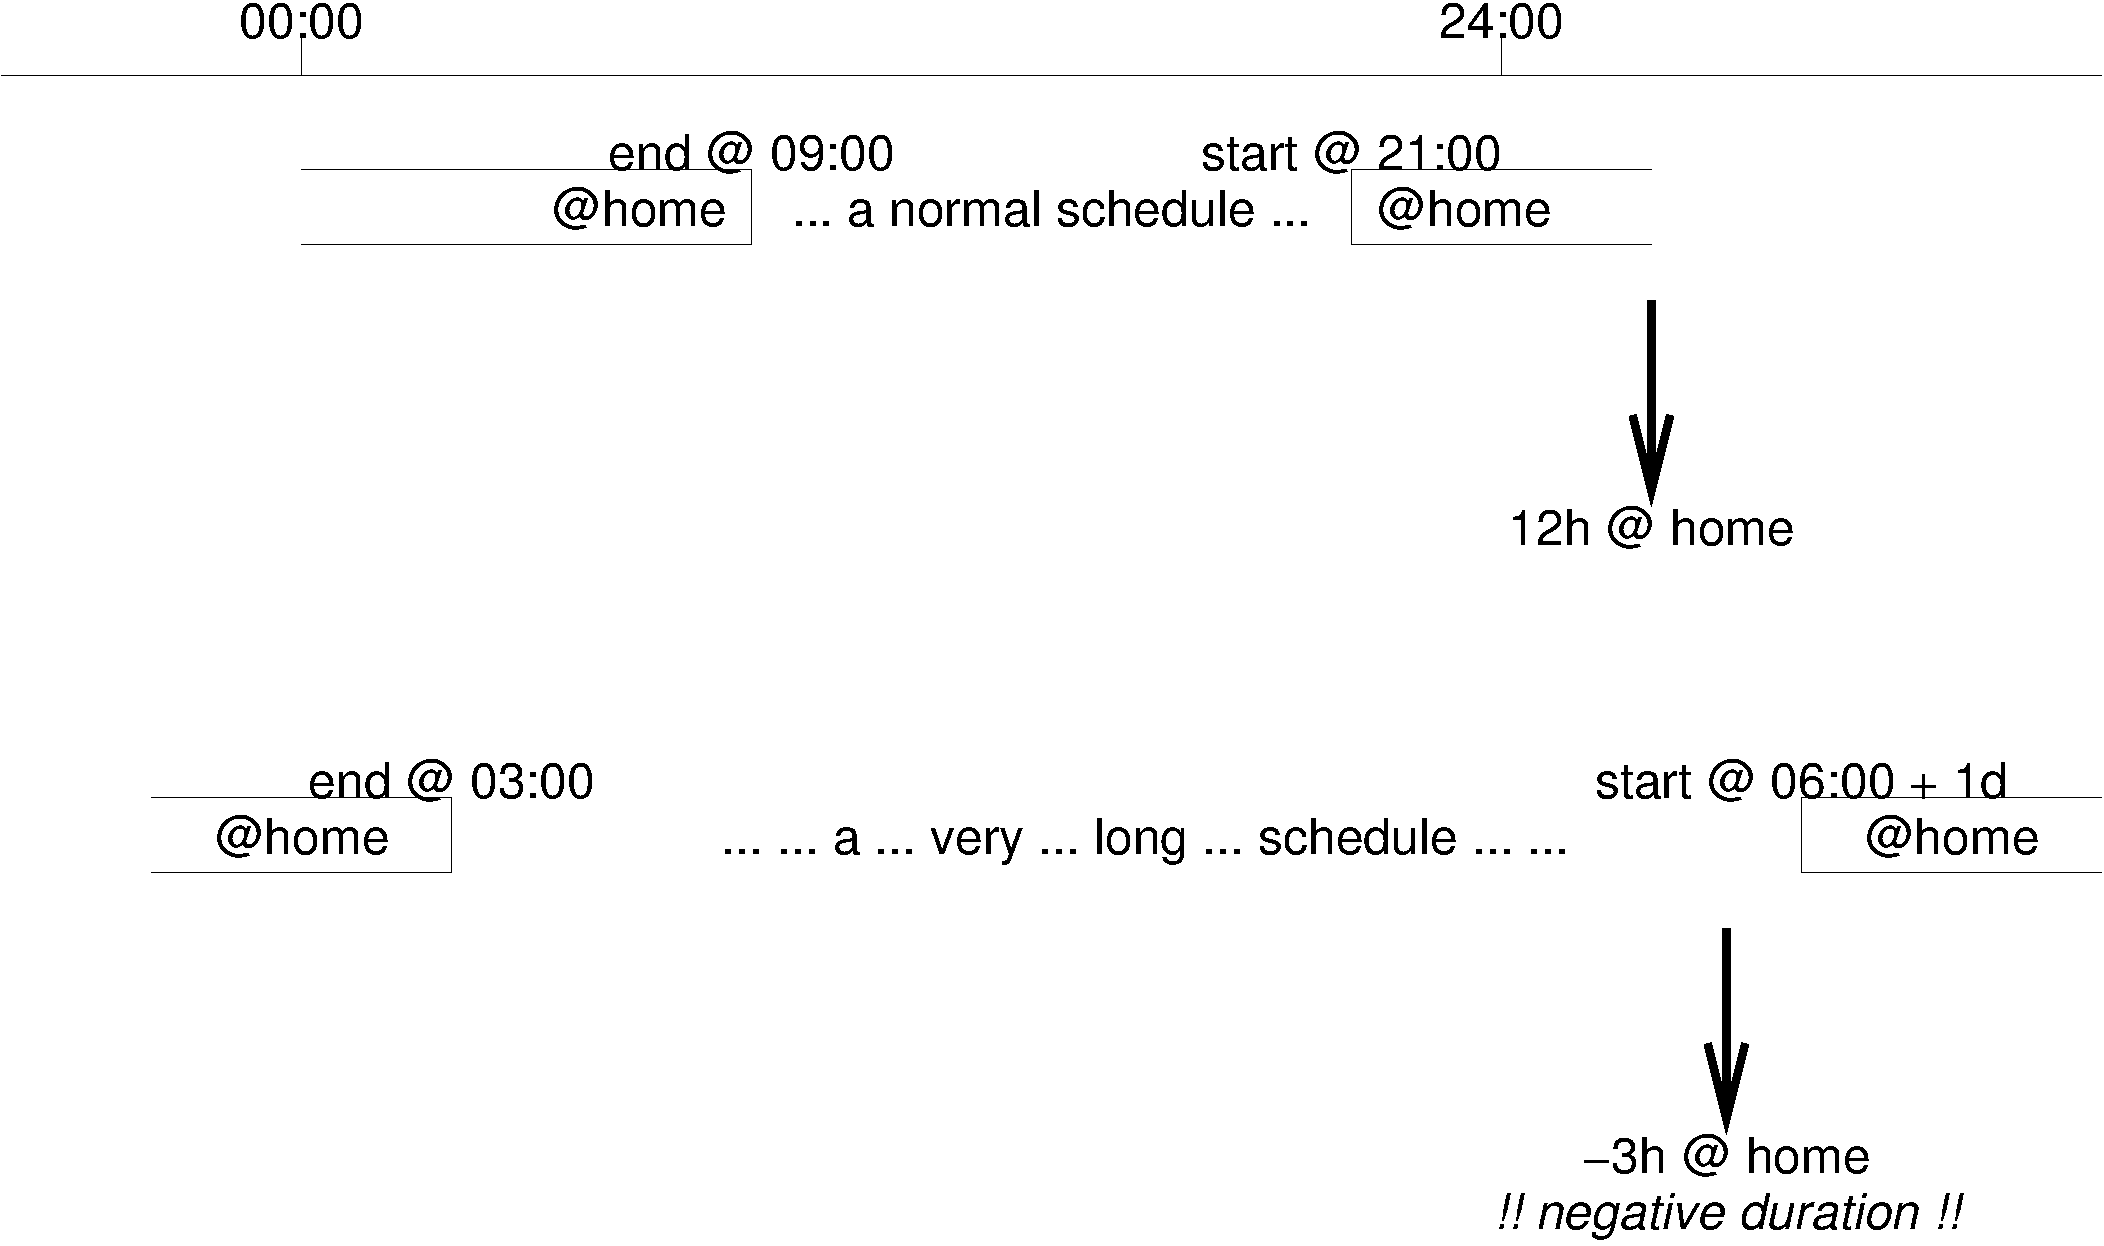
\includegraphics[width=0.8\hsize,trim=0 0 0 0,clip]{using/figures/negative-duration}}%
{}
% ------------

% ------------
\createfigure%
{Extending the slope when the utility function crosses the zero line to negative durations}%
{Extending the slope when the utility function crosses the zero line to negative durations}%
{\label{tab:score-extension}}%
{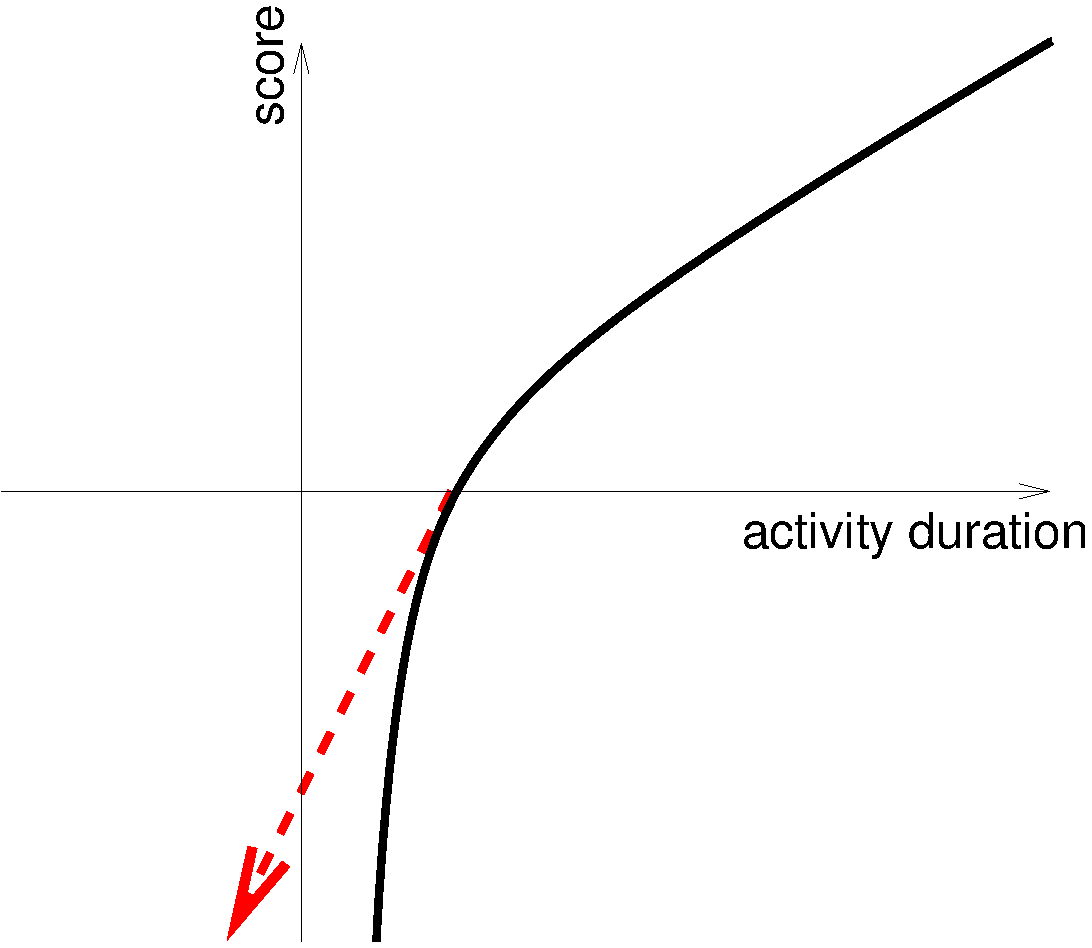
\includegraphics[width=0.4\hsize,trim=0 0 0 0,clip]{using/figures/score-extension}}%
{}
% ------------

\paragraph*{Negative Durations}

In \gls{matsim}, somewhat curiously it is possible to have activities with negative durations. This can happen because of the ``wrap around'' mechanism, where the last activity of a plan is stitched together with the first activity of the plan, and only that merged activity is scored (\cf Section~\ref{sec:wrap-around}). 
%% \kai{Der Ansatz, dass man alle Aktivitäten des selben Typs erst aufsummiert, würde dies hier natürlich auch lösen.}
In this situation,
% \kai{und auch wenn wir es anders machen würden!!}, 
it can happen that an agent arrives at the last activity of the plan at a later time-of-day than when the first activity ended.  Originally, a score of zero was assigned to such activities of negative duration. However, the adaptive agents quickly found out that they could use this to their advantage: Expanding this negative duration without a penalty would lead to more time elsewhere, which the agent could use to accumulate score. %% This is a bit similar to the question if a search algorithm should allow infeasible solutions during search, and in an adaptive algorithm needs to be penalized high enough so that does not occur.
%
For an adaptive \gls{algorithm}, such a penalty needs to be defined such that it guides the adaptation back into the feasible region. From this, it follows that the penalty needs to become larger with increasing negativity of the duration. It also needs to be larger, \ie more strongly negative, than any score value for a positive activity duration.  The latter is, however, impossible to achieve with a logarithmic form which tends to $-\infty$ as $t_{dur,q}$ approaches zero from above. The current approach is to take the slope of the expression $\beta_{dur} \cdot t_{typ,q} \cdot \ln( t_{dur,q} / t_{0,q} )$ when it crosses zero, and extend this towards minus infinity (Figure~\ref{tab:score-extension}).

\paragraph*{First and Last Activity not the Same}

Clearly, the wrap-around approach fails if the first and last activity are not the same.  The present code does not look at locations, but gives a warning and problematic results when they do not have the same type.

% ##################################################################################################################
\section{Parameters}
Two frequently applied starting points for utility function calibration are the parameter set proposed by \citet[][]{CharyparNagel2005ga4acts} and the estimates by \citet[][]{Kickhoefer_MastersThesis_2009}.

\citet[][p.393]{CharyparNagel2005ga4acts} recommend
\begin{equation}
  \begin{array}{lcrl}
\beta_{dur} & = & 6\, & utils/h \\
\beta_{trav, mode(q)} & = & -6\, & utils/h \\
\beta_{wait} & = & 0\, & utils/h \\
\beta_{short.dur} & = & 0\, & utils/h \\
\beta_{late.ar} & = & -18\, & utils/h \\
\beta_{early.dp} & = & -18\, & utils/h .\\
  \end{array}
\label{eq:std-params}
\end{equation}
(cf.~Equation~(\ref{eq:derivation-of-scoring-default})).
%% These parameters were derived from \citet[][]{ArnottEtAl_TAER_1993} by also consulting \citet[][]{ChaumetEtAl_2006}. 
%% \kai{Andreas, wieso Chaument?} 
\ah{So ganz direkt sind ja die Parameter weder von Arnott noch von Vickrey abgeleitet. Chef meinte, dass da nach langen Diskussionen, mit Chaumet (und M. Bernhard, damals am IVT) noch (nach-)kalibriert wurde. Leider lange vor meiner Zeit.

\citet[][p.164, p.173]{ArnottEtAl_TAER_1993} defines 
$\alpha=5.00\ \$/h$ the shadow cost of travel time,
$\beta=3.05\ \$/h$ the unit cost of arriving early at work, and
$\gamma=11.88\ \$/h$ the unit cost of arriving late based on the estimations reported by \citet[][Table 2 on p.473]{Small_AER_1982}.
Derived from this initial values \citet[][p.382]{CharyparNagel2005ga4acts} define the MATSim utility function as follows [...], where they consider the opportunity costs of $20\ EUR/h$, \ie the costs for doing nothing. 

Frage ist hier: wie genau kam man auf die Werte? 

In \citet[][p.122]{ArnottEtAl_JUE_1990}, they are defined as $\alpha=6.40\ \$/h$, $\beta=3.90\ \$/h$ and $\gamma=15.21\ \$/h$.

%Bernhard and Axhausen: Metaanalysis. Normwerk. Verlässlichkeit ...
% Chaumet, R., P. Locher, F. Bruns, D. Imhof, M. Bernard and K.W.\ Axhausen (2007) Verfahren zur Berücksichtigung der Zuverlässigkeit in Evaluationen, final report for VSS 2002/002, Schriftenreihe, 1176, %Bundesamt für Strassen, UVEK, Bern. 
}

\kai{Arrgghh.  Es ist doch erstaunlich, wie Legenden entstehen können (in dem Fall die Legende, dass 6/12/18 ``the typical Vickrey parameters'' seien); offenbar hat das nie jemand nachgeschaut, inklusive mir selbst.

  Vickrey selber hat 0ct/min für trav, 1ct/min für wait, 2ct/min für perf und 4ct/min für late.  Habe das jetzt nicht gelesen, aber auch das scheint die Opportunitätskosten der Zeit somit separat auszuweisen; wenn man das integriert, dann hat man 2ct/min für traf\_eff, 3ct/min für wait\_eff und weiterhin 4ct/min für late.  Hm.

  ---

  Bei CharyparNagel müsstest Du auch noch in Section 8 reinschauen, da stehen die derzeitigen 6/12/18.

  ---

  Meine Erinnerung ist wie folgt:

  Ich bin mir ziemlich sicher, dass ich die beiden Arnott-et-al papers damals schon kannte (hatte ich in Los Alamos schon gelesen).  Kann aber nicht sagen, ob ich David Charypar die Werte 6/12/18 direkt gegeben habe, oder ob er sie aus dem Paper extrahiert hat.

  Benjamin hat das dann mal nachgeschätzt (darauf bezieht sich der Absatz unten; eigentlich müsste es aber m.E.\ Tabelle 5 sein).  Seine Werte (perf/car/wait/late = 2.26/0/0/-11) waren deutlich anders (matsim hat 6/-6/0/-18), aber die verkehrlichen Resultate schienen, soweit wir sehen konnten, nicht anders, insbesondere nicht besser im Vergleich mit Zählungen.

  Außerdem hat car=wait=0 zur Folge, dass das Arnott/Vickrey bottleneck model nicht mehr funktioniert, weil im Auto sitzen dann auch nicht mehr schlechter als zu früh kommen ist.  Inhaltlich scheint das (sogar) plausibel, aber vom Gefühl her wird ein solches Modell instabil.

  Schlussendlich ist ``wait'' schwierig zu schätzen, weil die meisten Befragungen das nicht sauber abfragen.

  Wir hatten dann beschlossen, den matsim-default bei 6/12/18 zu lassen, weil dies zum einen plausible Resultate gibt, und weil die sehr synthetischen Werte deutlich machen, dass man die Werte eigentlich anpassen müsste.

  ---

  Besonders schlimm finde ich das jetzt nicht.  Wir sollten allerdings das wording vorsichtiger gestalten (``loosely based on Vickrey/Arnott'').  Und aus meiner Sicht hat Chaumet da nichts zu suchen; da müsstet Ihr wissen, welche Rolle er da gespielt hat.

}

\citet[][]{Kickhoefer_MastersThesis_2009} added monetary variables and income to the \gls{matsim} utility function and performed a mode-specific estimation based on the survey by \citet[][]{VrticEtAl_ResRep_SVI_2007}. The utility function extended by monetary factors was linear, both in the variables and the parameters. Estimated parameters are given in Table 3 of \citet[][]{Kickhoefer_MastersThesis_2009}. The income-dependent utility function was based on \citet[][]{Franklin_PhDThesis_2006}.

%% Note, that nowadays the utility function measures in the unit $utils$, where an earlier interpretation was based on monetary terms (e.g., $\EUR$).
%
%m.E. nicht notwendig.  kai, jan'2015

% ##################################################################################################################
\section{Applications and Extensions}
\label{sec:appsExtensions}

\kai{do we need to mention the change to events-based scoring here?  revise ...}
The default scoring function has been applied and extended for various purposes. Please be aware, that the \gls{matsim} code base and in particular the scoring functionality has changed a lot in recent years, \eg the scoring is now based on events rather than on plans as it was the case before revision r17026 in October~2011.
%\ah{Btw: when exactly (revision?) did we switch to events-based scoring? Is relevant in other chapters too.}
%\kai{MZ should know this.}
%\thibaut{plan elements from the plans stopped being passed to the scoring function from r17026 on (24 Oct 2011).}
Thus, the historical development is accompanied by various conceptual and technical modifications leading to the current utility function described above. This also means, that the reported parameter settings in the literature are an indication not a direct recommendation.

Important applications for large scenarios are described in Chapter~\ref{ch:scenarios}.

Special utility functions have been developed for car sharing (see Chapter~\ref{ch:carsharing}), social contacts and joints trips (see Chapter~\ref{ch:jointtrips}), parking (see Chapter~\ref{ch:parking}), road pricing (see Chapter~\ref{ch:roadpricing}), and destination innovation (see Chapter~\ref{ch:destinationchoice}), also describing facility loading scoring and inclusion of random error terms. 
 
Future topics, available in an experimental manner, are a full-blown utility function estimation (Section~\ref{sec:estimation}), inclusion of agent-specific preferences (Section~\ref{sec:agent-specific-prefs}), and application of alternative utility function forms (Section~\ref{sec:alternative-functions}).

% ##################################################################################################################
%\section{Discussion}
%\label{sec:discussion_scoring}
%Will be commented, when chapter is finished. Make final results traceable.
%
%% =====================================================================================
%\subsection{Nutzenfunktion}
%\label{sec:utfd}
%
%
%\benjamin{noch was (relativ wichtiges):
%
%Wir notieren die Nutzenfunktionen in MATSim immer als $V_{i,car} = ...$ etc. Ich würde sehr empfehlen, das im Buch auch so zu machen.
%
%Habe gerade (im noch nicht committeten economic eval Kapitel folgenden Kommentar von mir gesehen, und dachte ich teile das mal:
%
%"I would strongly recommend to use $V_p$ instead of $S_p$ for an agent's plan even though this is not entirely the same as in Discrete Choice Theory, since some of the $\varepsilon$ is already captured by the simulation noise that Gunnar called $\eta$...In consequence, the score is NOT equal to $V_p$. 
%We should explain that in more detail."
%
%Bei deinen frozen epsilon und BestSelect ist $S_{}$ dann zwar wahrscheinlich richtig, aber so wie es jetzt in dem Kapitel über Charypar-Nagel steht ist es m.E. falsch.
%
%Was meinst du/ihr?
%}
%
%\gunnar{ja, zugestimmt. Vielleicht
%
     %\[U = V + eps\]
%
%wie üblich beibehalten und dann
%
     %\[V = \sum_i b_i E\{x_i\}\]
%
%schreiben, wobei $x_i$ weiterhin stochastische Attribute aus der mobsim sein können (und der Erwartungswert-Operator bei deterministischen Attributen ja nicht schadet). Das ist dann vermutlich auch konsistent mit der Weise, auf die die Modelle geschätzt wurden. Das eps würde dann alles mögliche absorbieren können (gumble, frozen, mobsim).
%}
%
%
%\ah{Dinge, welche man m.E. dabei irgenwie noch einbeziehen müsste:
%
%-$\varepsilon$ gibt es explizit momentan nur für Destination Choice (Mail Gunnar).
%
%-ohne $E\{.\}$ ist man mit $S_{}$ wohl mindestens so nahe an der Wahrheit dran wie mit $V$ (wegen $\eta$) (Mail Benjamin).
%
%- Konsistenz: in sehr vielen Publ. kommt seit Jahren $S_{plan}=S_{act}+S_{travel}$ vor. Könnte mir vorstellen, dass gerade neue User verwirrt sind, wenn wir davon abrücken (ohne grosse Not?-> $\eta$!).
%}
%
%\ah{Gunnars Mail doch noch kapiert. So müsste es gehen.}
%
%% =====================================================================================
%\subsection{Score and Its Interpretation}
%\label{sec:scored}
%\kai{
%Die ursprüngliche Aussage war: 
%
%(1) Matsim produziert einen "score", analog einer "fitness" in evolutionary algorithms.  Notiert als "S".
%
%(2) Wie das dann interpretiert wird, ist ein zweiter Schritt. (Z.B. ob als U oder als V.)
%
%
%IVT argumentiert, dass sämtlicher Noise durch die Simulation erzeugt wird, und verwendet "SelectBest" bei choice.  Dann ist U = S.  (Also: Aller Nutzen des Agenten kommt aus dem Score.)
%
%VSP verwendet ein logit model bei choice ... und argumentiert damit letztendlich (aber bisher nicht absichtlich), dass beim choice \textbf{weiterer} (durch den scale parameter parametrisierter) noise hinzugefügt wird.  Dann ist U = S + epsilon .   (Wichtig: Es gibt Nutzen für den Agenten über den Score hinaus.)
%
%
%Für den zweiten Fall gilt Gunnars Theorie von conceptual meeting: "one can only convincingly claim that S = V when S is an expected value".
%
%Ich weiß gar nicht, was für den ersten Fall gilt.
%
%
%Kohärent aufschreiben kann man das m.E. nur, indem man konsistent bei "S" bleibt, und den Schritt der Interpretation separiert von dem, was MATSim tut.
%
%
%Wie jetzt weiter?
%
%
%(a) matsim output konsistent als "S" notieren statt "U" oder "V"?
%
%(Der Latex-Aufwand würde sich m.E. in Grenzen halten; es wäre m.E. die konsistenteste Lösung; fraglicher wäre die Lesbarkeit.)
%
%
%(b) bei "U" bleiben, aber Fußnoten dranmachen im Sinne von "matsim agent-based score is loosely interpreted as agent-based utility; for a discussion and relation to discrete choice see Chap XY and YZ".
%
%
%(c) weitere Vorschläge?
%
%
%Ich bin auf jeden Fall derzeit skeptisch, ob wir wirklich alle U nach V umwandeln sollen, und ich bin auch skeptisch, ob wir bereits im "using" Teil überhaupt von U = V + eps sprechen wollen.
%
%
%Kommentare?  Meinungen?
%
%}
%
%\gunnar{ich möchte meine Antwort hierauf gerne ein paar Stunden, max einen Tag, aufschieben und das "choice models in matsim" Kapitel entsprechend formulieren.}
%
%\ah{Bin nicht sicher, ob das hier am IVT tatsächlich alle machen, oder nur ich, wenn ich das Best-Response-Modul Destination Choice anwerfe. Ich jedenfalls nehme auch Logit, wenn ich keine Destination Choice mache.
%
%Bis zu Gunnars Kapitel bei "S" bleiben und dann erst den Link zu Discrete Choice machen, fände ich eine gute Lösung. Man müsste im Scoring-Kapitel (und Glossar) dann halt kurz erklären warum wir jetzt plötzlich nicht mehr wie alle die Jahre "U", sondern vorerst mal "S" schreiben. U=V+eps ist ja eigentlich in den ersten beiden Teilen nur für Zielwahl wirklich relevant, und das kriege ich dann schon auf Gunnars Kapitel angepasst.
%
%Verständnisfrage: Die Aussage gilt nur für Random-Mutation-Settings, oder? Für Route-Choice, z.B., wird bloss das Konvergenzverhalten beeinflusst, oder? }
%
%\kai{
%Leider keine einfache Sache, siehe auch unsere Kapitel über econ eval. 
%
%(A) Was macht matsim derzeit?
%
%(1) Ein choice model $\exp(V_i) / \sum_j \exp(V_j)$ impliziert einen echten Nutzen von U = V + eps .
%
%(2) Der erwartete (= mittlere) Nutzen ist dann der logsum term:  $E(U) = ln \sum_j \exp(V_j)$
%
%(3) Ordnen wir die Pläne so, dass der Plan mit dem höchsten Nutzen die Nummer 1 ist.  dann
%
%$ln \sum_j \exp(V_j) = ln ( \exp(V_1) * ( 1 + \sum_{j \ge 2} \exp(V_j - V_1) ) = V_1 + ln( 1 + ... )$
%
%Das ist offensichtlich größer als $V_1$; der mittlere Nutzen ist größer als der höchste Score!
%
%So geht das ganz generell: Die Hinzufügung weiterer Pläne, selbst wenn sie schlechter sind als der beste, erzeugen bei diesem Ansatz zusätzlichen mittleren Nutzen.
%
%Das gilt auch dann, wenn sich die zusätzlichen Pläne nur in der Route unterscheiden.
%
%
%(B) Ist das sinnvoll?
%
%Fraglich.  Oft hat matsim am Ende der Iterationen 5 identische Pläne; die erzeugen dann in der Rechnung $ln(5)$ an zusätzlichem Nutzen; das ist aber auch formal nicht richtig, weil vollständig korrelierte Optionen nicht zum Nutzen beitragen dürfen.  Gunnar wird vielleicht einwenden, dass man hier "path size logit" verwenden sollte ... 
%
%... ich selber würde inzwischen sagen, dass ich finde, dass das zu kompliziert wird.  Die Schönheit des agenten-basierten Ansatzes war doch, dass dass man auch ohne solche statistisch komplizierten Argumente auskommt.
%
%
%(C) Was tun?
%
%Mittelfristig ist das eine Forschungsfrage.  Ein erster Ansatz wäre u.E. eine Variante Deiner frozen epsilons auch für andere Situationen.  Jeder neue Plan kommt dann zusammen mit einem neuen frozen epsilon, wobei die Bandbreite sich eigentlich daran orientieren müsste, wie sehr sich dieser Plan von anderen Plänen unterscheidet.  Dann z.B.:
%
%* nur neue Route -- frozen epsilon wird übernommen
%
%* ...
%
%* neue location -- frozen epsilon stammt aus Horni-Ansatz
%
%Damit ist dann klar, dass der Agent einen $score > V_best$ erhalten kann; das geht ja bereits bei Deinem Paper so.  Aber alle epsilons ist dann bereits im "S" drin, und der Score, den matsim ausspuckt, ist dann einfach nur der tatächliche Nutzen, den der Agent erhält.
%
%(Leider weiß ich nicht, was das mit Cadyts macht, aber man könnte behaupten, dass Cadyts halt genau die frozen epsilons kalibriert.)
%
%
%Nun ja.  Wolltest Du es so genau wissen?  :-)
%
%}
%
%\kwaah{
%danke, soweit ich mich erinnere (siehe Ben-Akiva und Lerman) ist der log sum Term der maximale Nutzen ueber alle Alternativen, d.h. solange die Alternativen nicht identisch
%sind, erhoeht eine wahre zusaetzliche Alternative den Nutzen des Satzes der Alternativen. 
%
%Das ist auch das Argument hinter der Nutzung des log sum terms als Wohlfahrtsmass. 
%}
%
%\gunnar{
%Es gilt in beiden Fällen, so war es ja konstruiert. Kombiniere U = S (1. obiger Abschnitt) und S = V (3. Abschnitt); das liefert U = V. Da $V=E\{U\}$ per Definition, gilt das weiterhin nur, wenn U (also S im 1. Abschnitt) ein Erwartungswert ist.
%
%> bereits im "using" Teil überhaupt von U = V + eps sprechen:
%
%Nur S im "using" Teil, mit einem Verweis auf Teil 3.
%}

% ##################################################################################################################
%\section{Extensions}
% ======================================================================================================================
%\paragraph{Project Westumfahrung Zürich:}
%Project Westumfahrung \citep[][]{BalmerEtAl_ResRep_bdktzrh_2009} used the Zürich scenario version 1 \citep[][]{HorniEtAl_TechRep_IVT_2011_a}. Only car traffic was simulated with $\beta_{perf,q}=6.0\ utils/h$ and $\beta_{trav,q}=-6.0\  utils/h$. No further penalties were applied. Typical activity durations were provided with the config with half-hour resolution and empirically derived from the Swiss microcensus.

% ======================================================================================================================
%\paragraph{Project Location-Based Services:}
%\citet[][]{BalmerEtAl_ResRep_datapuls_2010} was simulated on the Swiss scenario version 2 \citep[][]{HorniEtAl_TechRep_IVT_2011_a}. Innovations related to the utility function are agent-specific typical activity durations and facility-specific opening hours. Summation of activity duration for activities of the same duration (denoted as $S_{cum}$) was added by \citet[][p.9 and p.28]{BalmerEtAl_ResRep_datapuls_2010}. Facility-loading penalties were included as detailed below. The parameters \citep[][Table 2 on p.31]{BalmerEtAl_ResRep_datapuls_2010} of the multi-modal utility function including monetary costs was heavily based on the estimates by Kickhöfer \citep[][]{Kickhoefer_MastersThesis_2009}. Egress and access times to and from public transport stops was included, public transport travel times were not simulated but imputed. Due to problems with spreading of many plans into the next day a penalty for too long day plans was added.

% ======================================================================================================================
%\paragraph{Project Herbie Mode Choice:}
%Project Herbie \citep[][]{VitinsEtAl_VW_2012} provided a thorough calibration of the multi-modal Zürich scenario extended by public transport simulation, cross-border and freight traffic, tolling, parking pricing, park \& ride and joint riding. The mode-share calibration targeting on distances and shares was based on the Swiss microcensus \citep[][p.18]{VitinsEtAl_VW_2012}.   

% ======================================================================================================================
%\paragraph{Project Tel-Aviv:}
%\citet[][]{BekhorEtAl_TRB_2011, DoblerEtAl_TechRep_IVT_2014} combine MATSim with the Tel-Aviv activity-based model \citep[][]{CambrigeSystemsInc_ResRep_TelAviv_2008}. Its multi-nomial zone-based utility function is integrated into MATSim by disaggregating the zones into facilities.

% ======================================================================================================================
%\paragraph{Singapore:}
%In the Singapore scenario \citep[][]{ErathEtAl_IATBR_2012} the basic multi-modal Charypar-Nagel utility function is applied. Its parameters derived from the Singapore Land Transport Authority (LTA) model. The utility function is measured in SGD rather than utils.

% ======================================================================================================================
%\paragraph{Car Sharing:}
%\citet[][p.10]{CiariEtAl_TechRep_IVT_2014} used the following car sharing specific utility function terms: access and egress time costs for walking, monetary cost of distance, and rental costs (constant and time-dependent). Simulations were performed for the multi-modal Zürich scenario with the parameter set described in Table 1.
%
% ======================================================================================================================
%\paragraph{Parking:}
%\citet[][]{WaraichAxhausen_TechRep_IVT_2012} extended the utility function by a parking term including walking to and from the parking lot (p.7) and parking costs (p.9). Simulations were run for the Zürich car traffic scenario. \citet{WaraichEtAl_unpub_TRB_2013} implemented a parking location choice model based on parameters estimated by \citet[][]{WeisEtAl_TechRep_TSMS_2013}.
%
% ======================================================================================================================
%\paragraph{Road Pricing:}
%Road pricing is a MATSim extension. It can be added by an event listener to the controler. The utility function then gets money events, converts them, and accumulates them to the rest of the score which is given in utils.
%
% ======================================================================================================================
%\paragraph{Social Contacts and Joint Trips:}
%There are two approaches modeling social contacts in MATSim, \citet[][]{Hackney_PhDThesis_2009} and the work performed by Thibaud Dubernet. Both modify scoring in a similar way; by increasing each individuals score if they coincidently perform an activity of the same type in the same facility. Both restricted the type to leisure to begin with. Dubernet also includes joint car rides in that calculation; but sometimes instead the marginal utility of travel is modified (Thibaud Dubernet, personal communication, March 2014). Linear and logarithmic functions have been tried by Dubernet, where recent experiments showed that, as expected, a logarithmic function increases the number of friend contacts, giving the microsimulation user another calibration parameter. 
%
% ======================================================================================================================
%\paragraph{Destination Choice:}
%Goal of the estimation described by \citet[][]{Horni_PhDThesis_2013} were first indications about quantitative relation of MATSim time parameters and further choice attributes. Focusing on destination choice, attributes used for estimation were \emph{store size} (in categories), \emph{price level} (in categories) and \emph{additional linear distance} to the store similar to the detour distance defined in \citet[][]{ArentzeTimmermans_TRR_2007}.
%
%Clearly, for direct application in MATSim, travel times rather than distances would have been better, but this information was not available consistently. A minimal set of variables was chosen due to data availability and as the main goal was laying an instructive base for future MATSim utility function estimations and their application in the MATSim Zürich scenario. Alternative-specific constants were not assigned to destinations to prevent over-fitting \citep[][]{BierlaireEtAl_TransScience_1997}.
%
%Although the estimated parameters had to be enlarged to show significant effects, their relation was correct as experiments with this extended and adapted model showed a surprisingly substantial decrease of the relative error in count data.
%
%Non-linear estimated models containing travel time are scarce as travel time is an unreliable information in surveys. A way to approximately applying simple linear distance models to the non-linear time-based MATSim utility function is discussed in Section 5.5.1 of \citet[][]{Horni_PhDThesis_2013}.
%

% ======================================================================================================================
%\paragraph{Agent-Specific Preferences:}
%In project Surprice \citet[][]{HorniEtAl_TechRep_IVT_2012_a, HorniAxhausen_TechRep_IVT_2014}, agent-specific travel preferences and individual income-dependent marginal utilities of money are incorporated. It is simulated with a 1\% multi-modal Zürich scenario, the preference values however, are assigned randomly.


% ##################################################################################################################
% Local Variables:
% mode: latex
% mode: reftex
% mode: visual-line
% TeX-master: "../main"
% comment-padding: 1
% fill-column: 9999
% End: 
